%!TEX TS-program = pdflatex
\documentclass[12pt]{article} %article
 
% The declaration of the document class:
\usepackage{amsmath}
\usepackage[english]{babel}
\usepackage{geometry}
\geometry{verbose,letterpaper,margin=2.45cm}

\usepackage[full]{textcomp}
\usepackage[T1]{fontenc}
%\usepackage{kpfonts}
\usepackage[utf8]{inputenc}
\usepackage{lineno}

\usepackage{pgfplots,pgfplotstable}
\usepackage{longtable}
\usepackage{booktabs}					 
					 
\setlength{\parindent}{0pt}
\setlength{\parskip}{6pt plus 2pt minus 1pt}
					 
\pagestyle{plain}
\usepackage{setspace}
 
% Table formatting:
% What if you make a table? -- Pandoc knows, of course, and
% then declares that its variable `table` is True and
% imports a table package suitable to its pleasantly simple tables.
% Needless to say infinitely complicated tables are possible in
% LaTeX with suitable packages. We are spared the temptation:
 
\usepackage{array}
 
% Continuing on the topic of tables ... (we havent reached `endif`).
% The commented out line below is in the default pandoc latex.template.
% Some unpleasantness with table formatting must be corrected.
 
% -- This is needed because raggedright in table elements redefines \\:
\newcommand{\PreserveBackslash}[1]{\let\temp=\\#1\let\\=\temp}
\let\PBS=\PreserveBackslash
 
 
 
% Subscripts:
% Pandoc remembers whether you used subscripts, assigning True to
% its `subscript` variable
% It then needs to adopt a default with an incantation like this:
 
 
% Web-style links:
 
% markdown inclines us to use links, since our texts can be made into html.
% Why not have clickable blue links even in
% learned, scientific, religious, juridical, poetical and other suchlike texts?
% Never mind that they have been proven to destroy the nervous system!
 
% First, what about the fact that links like http://example.com are
% technically code and thus must not be broken across lines?
% [breaklinks=true] to the rescue!
 
% Nowadays LaTeX can handle all of this with another half million macros:
 
\usepackage[breaklinks=true]{hyperref}
\hypersetup{colorlinks,%
	citecolor=blue,%
	filecolor=blue,%
	linkcolor=blue,%
	urlcolor=blue}
		
 
 
 
% Images.
% In ye olde LaTeX one could only import a limited range of image
% types, e.g. the forgotten .eps files. Or else one simply drew the image
% with suitable
% commands and drawing packages. Today we want to import .jpg files we make
% with
% our smart phones or whatever:
 
\usepackage{graphicx}
% -- We will generate all images so they have a width \maxwidth. This means
% -- that they will get their normal width if they fit onto the page, but
% -- are scaled down if they would overflow the margins.
\makeatletter
\def\maxwidth{\ifdim\Gin@nat@width>\linewidth\linewidth
	\else\Gin@nat@width\fi}
	\makeatother
	\let\Oldincludegraphics\includegraphics
	\renewcommand{\includegraphics}[1]{\Oldincludegraphics[width=\maxwidth]{#1}}
		 
	 

% Section numbering.
% Here again is a variable you can specify on the commandline
% `markdown2pdf my.txt --number-sections --xetex
% --template=/wherever/this/is -o my.pdf`

% Footnotes:
% Wait, didn't we already discuss the crisis of code in footnotes?
% Evidently the order of unfolding of macros required that
% we import a package to deal with them earlier
% and issue a command it defines now. (Or maybe that's not the reason;
	% very often the order does matter as the insane system of macro
	% expansion
	% must take place by stages.)

% Other stuff you specify on the command line:
% You can include stuff for the header from a file specified on the
% command line;
% I've never done this, but that stuff will go here:

% Title, authors, date.
% If you specified title authors and date at the start of
% your pandoc-markdown file, pandoc knows the 'values' of the
% variables: title authors date and fills them in.

\title{Relationships between environmental variabels and species richness}
\author{D. Li \and D. Waller}
\date{Working paper -- \today}

% At last:
% The document itself!:

% After filling in all these blanks above, or erasing them
% where they are not needed, Pandoc has finished writing the
% famous LaTeX *preamble* for your document.
% Now comes the all-important command \begin{document}
% which as you can see, will be paired with an \end{document} at the end.
% Pandoc knows whether you have a title, and has already
% specified what it is; if so, it demands that the title be rendered.
% Pandoc knows whether you want a table of contents, you
% specify this on the command line.
% Then, after fiddling with alignments, there comes the real
% business: pandoc slaps its rendering of your text in the place of
% the variable `body`
% It then concludes the document it has been writing.

% \setpagewiselinenumbers
\linenumbers

\begin{document}


\maketitle





\doublespacing
\textbf{Running headline}: Environment and species richness

\textbf{Abstract}: Your awesome abstract here.

\clearpage

\section{Introduction}\label{introduction}

Here is your introduction. It should describe clearly the rationale for
the study being done and the previous work related with the study. It
should also tell readers about your specific hypothese/questions being
addressed. Citations will be like this (Adair et al. 2010), or (e.g.,
Clark and Tilman 2008), or (Eriksson and Ehrlén 1993, Williamson et al.
1999)

\section{Methods}\label{methods}

Here is the method section. You can include equations easily. For inline
equations, use \(\text{var}(X) = p(1-p)\). For display equation, use

\begin{equation}
\text{var}(X) = p(1-p)
\end{equation}

\subsection{Results}\label{results}

Insert tables:

\begin{longtable}[c]{@{}rr@{}}
\toprule
Plot & sprich\tabularnewline
\midrule
\endhead
3294 & 31\tabularnewline
3297 & 28\tabularnewline
3299 & 26\tabularnewline
3330 & 27\tabularnewline
\bottomrule
\end{longtable}

Or put results inline, e.g.~the mean species richness is 28.

How about figures? We illustrate this in Fig. \ref{f:plot}.

\clearpage

\begin{figure}[htbp]
\centering
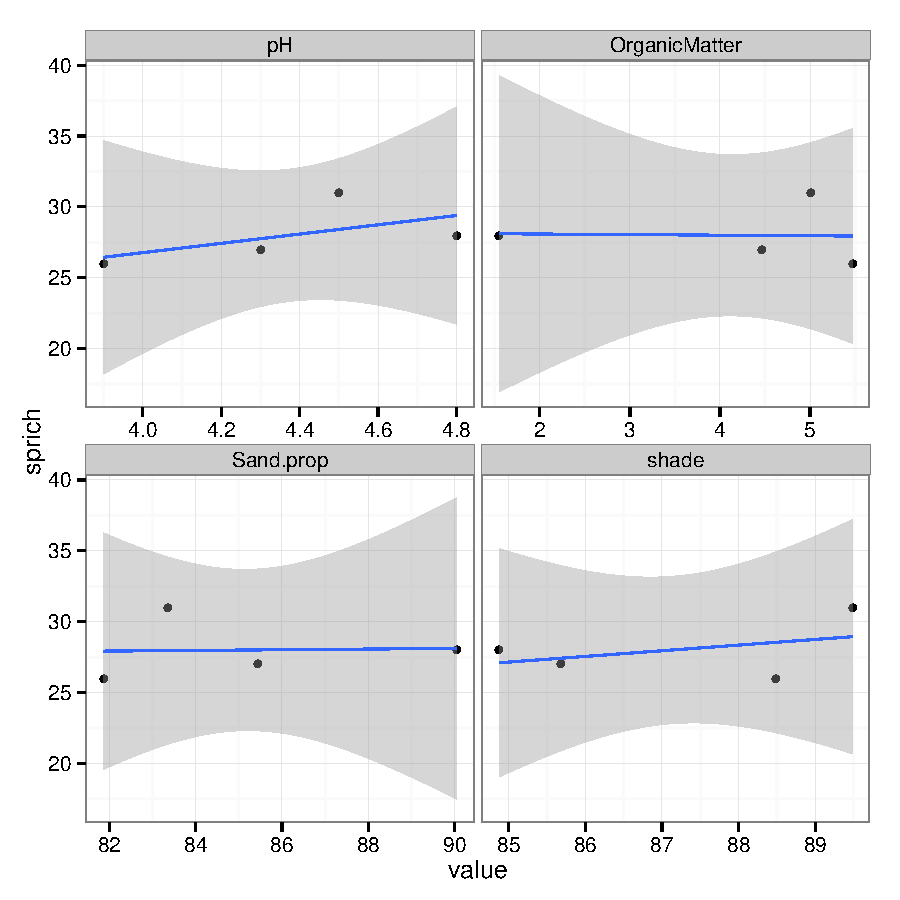
\includegraphics{Figs/plot.pdf}
\caption{Caption here.\label{f:plot}}
\end{figure}

\clearpage

\section*{References}\label{references}
\addcontentsline{toc}{section}{References}

Adair, E. C. et al. 2010. Single-pool exponential decomposition models:
Potential pitfalls in their use in ecological studies. - Ecology 91:
1225--1236.

Clark, C. M. and Tilman, D. 2008. Loss of plant species after chronic
low-level nitrogen deposition to prairie grasslands. - Nature 451:
712--715.

Eriksson, O. and Ehrlén, J. 1993. Seed and microsite limitation of
recruitment in plant populations. - Oecologia 92: 361--366.

Williamson, C. E. et al. 1999. Dissolved organic carbon and nutrients as
regulators of lake ecosystems: Resurrection of a more integrated
paradigm. - Limnology and Oceanography 44: 795--803.

%

\end{document}
